\subsection{Einstellungen}

\subsubsection{Aufgaben}
Die Anwendung, insbesondere die darin enthaltene Visualisierung, soll an die Bedürfnisse des Benutzers anpassbar sein. Die Einstellungen sollen sofort sichtbar sein. Weiters soll über den Einstellungen-Tab eine Verbindung zur GHI-Steuerung beziehungsweise SPS hergestellt werden können.

\subsubsection{Aufbau}
Um diese Aufgaben zu erfüllen wird ein eigener Einstellungen-Tab in der Oberfläche, sowie Data-Binding im Hintergrund verwendet. Dazu werden drei Klassen definiert - EdubotAdapterConfig, KebaAdapterConfig und VisualizationConfig - in denen die unterschiedlichen Einstellungen und Konfigurationen verwaltet werden. \\
Während die ersten beiden lediglich Informationen über die Netzwerkschnittstelle der Steuerung enthalten, ist die VisualizationConfig etwas komplexer aufgebaut. Die einzelnen Properties dieser Klassen sind an Eingabefelder des Einstellunge-Tabs gebunden und werden mit Hilfe sogenannter ValidationRules bei jeder Änderung überprüft und nur bei einem gültigen Wert geändert.

\subsubsection{Bedienung der Oberfläche}

\begin{figure}[H]
  \centering
  \begin{minipage}[t]{12 cm}
  	\centering
  	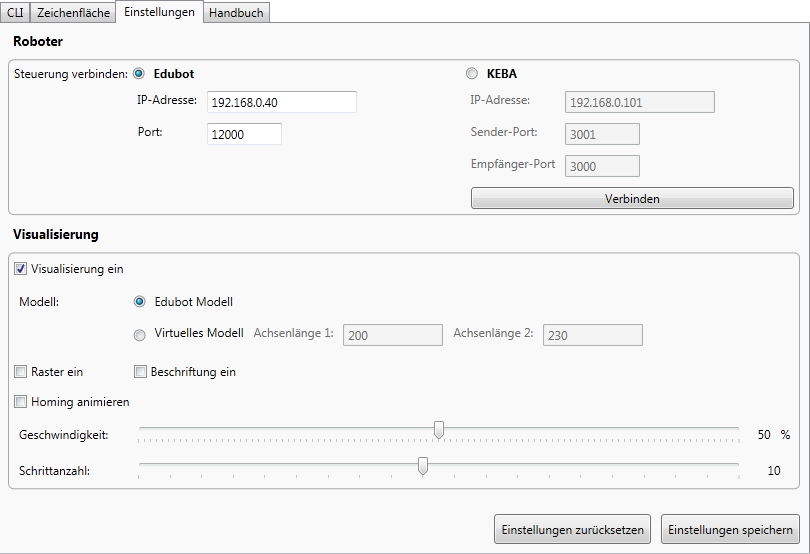
\includegraphics[width=12cm]{images/Settings} 
    \caption{Der Einstellungen-Tab}
  \end{minipage}
\end{figure}

Die Bedienung der Oberfläche ist realtiv einfach und leicht verständlich. Im oberen Bereich des Tabs befindet sich der "Roboter"-Bereich in dem eine der beiden unterstützten Steuerungen ausgewählt werden kann.\\ 
Unter den Namen dieser Steuerungen, befinden sich entsprechende Eingabefelder. Im selben Bereich befindet sich ein Button mit der Aufschrift "Verbinden", welcher nur angeklickt werden kann, wenn die eingegebenen Informationen gültig sind.\\
Klickt der Benutzer nun auf diesen Button, versucht die Anwendung eine Verbindung mit der Steuerung herzustellen. Dieser Vorgang wird in einem Fesnter dargestellt. Ist er erfolgreich so werden alle Elemente des Bereichs "Roboter", bis auf Button dessen Aufschrift nun "Trennen" lautet, deaktiviert. \\
Wurde der Edubot-Roboter verbunden, so wird das 3D-Modell entsprechend umgestellt und die Visualisierung auf die Längen des echten Modells angepasst. Solange der Edubot-Roboter verbunden ist, kann nicht auf ein anderes 3D-Modell umgestellt werden.\\
Erst durch einen Klick auf "Trennen" werden die deaktivierten Felder wieder aktiviert und es kann eine andere Steuerung verbunden beziehungsweise die 3D-Ansicht geändert werden.\\
\\
Im unteren Bereich die Sektion "Visualisierung", in welcher letztere auf die Bedürfnisse des Benutzers angepasst werden kann. Über mehrere Checkboxen kann die Visualiserung, die Homing-Animation sowie entsprechende Beschriftungen und Raster aktiviert oder deaktiviert werden. \\
Weiters kann über zwei Radio-Buttons ein 3D-Modell ausgewählt werden. Falls die das virtuelle 3D-Modell ausgewählt wird, so werden zwei Textfelder aktiviert in welcher die Länge der Achsen eingegeben werden kann.\\
Mit Hilfe von zwei Slidern kann die Genauigkeit des Rasters beziehungsweise der Beschriftung festgelegt und die Geschwindigkeit der Animation geregelt werden.\\
Über einen Speichern-Button im rechten unteren Bereich kann, bei gültigen Einstellungen, die aktuelle Konfiguration gespeichert werden. Außerdem können die Einstellungen über den Button "Einstellungen zurücksetzen" auf ihre Standardwerte zurückgesetzt werden.

\subsubsection{Umsetzung}
Um die Daten aus der Eingabemaske in die entsprechende Objekte zu übernehmen, müssen diese als DataContext des entsprechenden Controls gesetzt werden. Dies geschieht im Konstuktor der Anwendung, nachdem die Einstellungen geladen wurden.\\
Jedes Control ist über sein Binding-Property mit dem entsprechenden Property des DataContext-Objekts verknüpft. Dazu muss im Layout der Oberfläche angegeben werden, welches Property an das Control gebunden und wann eine Eingabe durch den Benutzer in das entsprechende Property übernommen werden soll. Um das Control über Änderungen des ihm zugewiesenen Properties zu informieren, implementiert die IConfiguration-Klasse das INotifyPropertyChanged-Interface. Dadurch erhält die Klasse ein PropertyChanged-Event, welches die entsprechenden Controls informiert. \\

\textbf{Validierung}\\
Einer Bindung können zusätzlich noch Validierungsregeln mitgegeben werden, die bei Änderung in der Eingabemaske den neuen Wert prüfen und nur bei gültigem Wert den Setter des Properties aufrufen. Um als Validierungsregel verwendet zu werden, muss eine Klasse von ValidationRule abgeleitet sein und die Validate-Methode implementieren. Letztrere gibt ein sogenanntes ValidationResult zurück, welche angibt ob der Wert und gültig ist und falls nicht eine entsprechende Fehlermeldung enthält\\
Von uns wurden folgende Validierungsregeln implementiert:
\begin{itemize}
\item \textbf{IPAddressValidationRule}\\
In der Validate-Methode dieser Regel wird geprüft ob der mitgegebene Wert folgende Bedingungen erfüllt:
\begin{itemize}
\item Der Wert darf nicht leer sein
\item Der Wert muss aus 4 Zahlen zwischen 0 und 255 bestehen
\item Die Zahlen müssen durch Punkte getrennt sein
\end{itemize}
\item \textbf{LengthValidationRule}\\
In der Validate-Methode dieser Regel wird geprüft ob der mitgegebene Wert folgende Bedingungen erfüllt:
\begin{itemize}
\item Der Wert darf nicht nicht leer sein
\item Der Wert muss eine Zahl sein
\item Die Zahl muss größer als 0 sein
\end{itemize}
\item \textbf{PortValidationRule}\\
In der Validate-Methode dieser Regel wird geprüft ob der mitgegebene Wert folgende Bedingungen erfüllt:
\begin{itemize}
\item Der Wert darf nicht nicht leer sein
\item Der Wert muss eine Zahl sein
\item Die Zahl muss zwischen 0 und 65535 sein
\end{itemize}
\end{itemize}
\textbf{IConfiguration}\\
Die abstrake Klasse IConfiguration dient dazu Code-Redundanz in den drei Config-Klassen zu vermeiden. Die Klasse enthält die Methode NotifyPropertyChanged, welche einen String mit dem Namen des geänderten Properties als Parameter übernimmt. In dieser Methode wird das PropertyChangedEvent mit entsprechenden PropertyChangedEventArgs ausgelöst. Die abgeleitenen Klassen EdubotAdapterConfig, KebaAdapterConfig und VisualizationConfig rufen diese Methode bei Änderung eines Properties mit dem Property-Name als Parameter auf.

\textbf{EdubotAdapterConfig}
Die EdubotAdapterConfig-Klasse enthält Informationen über die Netzwerkkonfiguration der GHI-Steuerung, welche für den Verbindungsaufbau nötig sind.
Eine Instanz dieser Klasse enthält folgende Properties:
\begin{itemize}
\item \textbf{IPAddress}\\
Das IPAddress Property enthält die IP-Adresse der GHI-Steuerung als String und ist entsprechend an ein Textfeld in der Maske gebunden. Es unterliegt der IPAddressValidationRule, welche neue Werte auf die oben angeführten Kriterien überprüft. Als Standard-Wert wird für dieses Property "'192.168.0.40"' vergeben.
\item \textbf{Port}\\
Das Port-Property enthält den Port auf dem unsere Steuerungssoftware läuft und ist ebenfalls an ein Textfeld im Einstellungen-Tab gebunden. Es unterliegt der PortValidationRule,  welche neue Werte auf die oben angeführten Kriterien überprüft. Als Standard-Wert wird für dieses Property "'12000"' vergeben.
\end{itemize}
Zusätzlich zu diesen Properties besitzt die Klasse noch die Methode Reset, welche alle Eigenschaften auf ihren Standard-Wert zurücksetzt.\\
\\
\textbf{KebaAdapterConfig}
Die KebaAdapterConfig-Klasse enthält Informationen über die Netzwerkkonfiguration der SPS, welche für den Verbindungsaufbau nötig sind.
Eine Instanz dieser Klasse enthält folgende Properties:
\begin{itemize}
\item IPAddress\\
Das IPAddress Property enthält die IP-Adresse der GHI-Steuerung als String und ist entsprechend an ein Textfeld in der Maske gebunden. Es unterliegt der IPAddressValidationRule, welche neue Werte auf die oben angeführten Kriterien überprüft. Als Standard-Wert wird für dieses Property "'192.168.0.101"' vergeben.
\item \textbf{SenderPort}\\
Das Port-Property enthält den Port auf dem die SPS Daten sendet und ist an ein Textfeld im Einstellungen-Tab gebunden. Es unterliegt der PortValidationRule,  welche neue Werte auf die oben angeführten Kriterien überprüft. Als Standard-Wert wird für dieses Property "'3001"' vergeben.
\item \textbf{ReceiverPort}\\
Das Port-Property enthält den Port auf dem die SPS Daten empfängt  und ist an ein Textfeld im Einstellungen-Tab gebunden. Es unterliegt der PortValidationRule,  welche neue Werte auf die oben angeführten Kriterien überprüft. Als Standard-Wert wird für dieses Property "'3000"' vergeben.
\end{itemize}
Zusätzlich zu diesen Properties besitzt die Klasse noch die Methode Reset, welche alle Eigenschaften auf ihren Standard-Wert zurücksetzt.ei Änderung eines Properties wird im entsprechenden Setter die Methode NotifyPropertyChanged mit dem Namen des geänderten Properties als Parameter aufgerufen. In dieser Methode wird das PropertyChangedEvent mit entsprechenden PropertyChangedEventArgs ausgelöst.\\
\\
\textbf{VisualizationConfig}\\
Die VisualizationConfig-Klasse enthält Informationen über die Darstellung der Visualisierung. Sie enthält ähnliche Properties wie der VirtualAdapter: Length, Length2, VerticalToolRange sowie MaxPrimaryAngle, MinPrimaryAngle, MaxSecondaryAngle und MinSecondaryAngle. Der Datentyp dieser Properties ist, durch das Data-Binding bedingt, String. Diese Informationen werden zum Initialisieren der VirtualAdapter in den verschiedenen Visualisierungen benötigt. Die VisualizationConfig stellt somit eine gemeinsame Datenbasis für das Erstellen dieser Adapter dar.
Zusätzlich zu diesen Informationen enthält die Klasse noch folgende, für die Animation und Darstellung relevante, Properties:
\begin{itemize}
\item \textbf{VisualizationEnabled}\\
Dabei handelt es sich um einen boolschen Wert, der angibt ob die Visualisierung aktiviert oder deaktiviert ist. Von diesem Property hängt ab, ob die Visualisierung einen VirtualAdapter bei der API registriert. Dieses Property ist an eine Checkbox im Einstellungen-Tab gebunden.
\item \textbf{ShowGrid}\\
Ein boolscher Wert der angibt ob das Gitter in der 2D-Animation angezeigt werden soll. In wie viele Schritte das Gitter unterteilt ist, wird durch das Steps-Property definiert. Dieses Property ist an eine Checkbox im Einstellungen-Tab gebunden.
\item \textbf{ShowLabels}\\
Ein boolscher Wert der angibt ob das Koordinaten-System der 2D-Animation beschriftet sein soll. Die Anzahl der angezeigten Koordinaten pro Achse, ist erneut vom Steps-Property abhängig. Dieses Property ist an eine Checkbox im Einstellungen-Tab gebunden.
\item \textbf{Speed}\\
Das Property Speed enthält einen Wert zwischen 1 und 100 und definiert die Geschwindigkeit in Prozent der Maximalgeschwindigkeit, mit der die Animation abläuft. Dieses Property ist an einen Slider im Einstellungen-Tab gebunden.
\item \textbf{Steps}\\
Das Steps-Property gibt an, in wieviele Teile jeder Quadrant des Koordinatensystems der 2D-Animation bei der Anzeige geteilt ist. Dieses Property ist an einen Slider im Einstellungen-Tab gebunden.
\item \textbf{IsEdubotModelSelected}\\
Dieses Property vom Typ Boolean definiert, welches 3D-Model ausgewählt ist. Ist es auf true gesetzt, so wird derzeit die Visualisierung des Edubot-Modells verwendet, andernfalls eine abstrakte dreidimensionale Darstellung eines Roboters. Dieses Property ist an einen Radiobutton im Einstellungen-Tab gebunden.
\item textbf{AnimateHoming}\\
Je nach Vorliebe des Benutzers kann die Animation vor Durchführung der Befehle die Homing-Phase eines Roboters animieren. Ist dieser Wert auf false gesetzt so startet die Animation bei einem Klick auf "Ausführen" sofort am Startpunkt, andernfalls fährt der Roboter erst zum Anfangspunkt und beginnt erst danach mit der Ausführung der Befehle. Dieses Property ist an eine Checkbox im Einstellungen-Tab gebunden.
\end{itemize}
